\documentclass{article}

% Any word on if they prefer IEEE journal format or old ES401?
% Don't worry about formatting - when the content is in I can
% do formatting by setting up a style file. 

\usepackage{graphicx}
\usepackage[utf8]{inputenc}
\title{ew401-fa2020-roboroach}
\author{A. Pak and B. D. Pritchard\thanks{Authors are with the Department of Weapons, Robotics, and Control Engineering at the United States Naval Academy}}
\date{September 2020}

\begin{document}
\maketitle

\begin{figure}[ht!]
\centering

\includegraphics[scale=0.5]{logo.png}

\label{fig:logo}
\end{figure}

\begin{abstract}
Abstract will go here eventually.
\end{abstract}

% If it is easier, we can split these into different files to make
% it quicker to find the right bit to edit too. 
\section{Customer Interview and Additional Background Research}
\subsection{Customer Background}
\par The Roboroach Capstone customer is Professor Levi Devries, a professor in the WRC department. Professor Devries was a double major in Physics and Math and also got his Masters in Aerospace Engineering from UMD. Though his experiences with Biomechanical projects are few and far between, Professor Devries is very interested in developing a new lab in the WRC curriculum because he wants to reinforce ideas being taught in early level courses while providing a new and helpful lab. From our first interview, we delved deeper into this idea, discussing how we could offer a lab in the early curriculum as well as a follow on to the 1/C EW485E Biomechanics elective. We also developed our initial thoughts for our functionality, metrics, and objectives. During our second interview, we finalized our top four metrics which were: simple, short duration, relevancy, and statistical significance. 



\subsection{Additional Related Research}
\par The RoboRoach project is something that could be extremely beneficial in the Biomechanics realm as well as in everyday life. If we could program insects and control their motions or even have computer vision through the insects, we could use them in the military to carry out reconnaissance missions that would be too dangerous for humans. This could also be used in so many different concetrations, practicing controlling robots and having them do certain tasks. Our background research mostly focused on related projects that shared similar inspiration with our project. 

% To make a new paragraph either skip a line or do \par
% Also I'll help you guys do citations etc so don't worry about fixing those yet
\par As to related works, the first related project we researched referred to controlling cows with virtual fencing. In ``Virtual Fences for Controlling Cows'', a team developed a moving virtual fence algorithm to herd cows \cite{butler2004virtual}. The intended market for this product is animal farmers or anyone who might need to herd animals. Because herding is a very labor intensive activity, the product aimed to eliminate the need for physical fences on farms. Their virtual fence methodology can be used to monitor grazing behavior in order to create models that lead to better land and pasture utilization, effectively optimizing the resource utilization, providing automation support, and easing the activities of animal farmers. The team made a smart collar for each cow in the herd, equipped with GPS, PDA (computer), wireless networking, and a sound amplifier. The animal is given the boundary of a virtual fence as a polygon specified by its coordinates and the GPS tracks its location against the polygon. As the animal approaches the boundary, a sound stimulus whose volume is proportionate to the distance from the boundary goes off. The team created static boundaries for grazing by leaving the polygon boundary as is, and dynamic boundaries for herding by slowly moving the polygon boundary in the desired direction. One lesson learned for our project is that the current moving speed of the test subject may influence the effect of the stimulus. Another lesson learned is that there are numerous ways to stimulate movement, such as emulating a behavior of a natural predator. We may incorporate the same approach with data collection as the team did, in that we would time how long it took the test subject to respond to the stimulus in the way we desire, but also take into account how often they respond in the way we desire. We did not see any specific shortcomings that they should have avoided or that we should avoid in the future. 

\par The second research article we looked was relating to controlling Hawkmoths. In ``Wireless Stimulation of Antennal Muscles in Freely Flying Hawkmoths Leads to Flight Path Changes'', the team used radio controlled, programmable, miniature stimulators to alter the pitch angle, flight speed, and flight altitude of hawkmoths \cite{hinterwirth2012wireless}. Though the intended user or market is not specified in the article, we believe that this product would appeal to researchers looking for a deeper understanding of neurophysiology within insects and subsequently humans. The goal of this product was to alter the flying behavior of a hawkmoth by stimulating its antennal mechanosensors. The team used \emph{Manduca sexta}, hawkmoths, as their test subject. Electrical stimuli were delivered to extrinsic antennal muscles via tiny electrodes injected to a dorsomedial location near each antennal rim. A miniature stimulator board delivered 2.8-3V square-pulse signals of 50 percent duty cycle and varying frequencies. A transmitter, communicating with the stimulator board wirelessly, was connected to a computer running software that stipulated the antennal muscles every 5 seconds. A high-speed video camera filmed the moth, and the team used a custom MATLAB digitizing software to extract the tip and base coordinates of the stimulated antenna and calculate deflection angles for each frame. One lesson learned for our project is that, at least for hawkmoths, stimulation of extrinsic muscles leads to antennal deflections while at rest. This article implies that this is true for all creatures with antennae, so we can expect similar results with a cockroach. Another lesson learned is that variation in electrode placement leads to slightly different recruitment of mechanosensors, so we will be extremely precise and deliberate in our measurements before we insert electrodes. The electrical stimulation aspect of this experiment will be very similar to that of ours. We will attempt to stimulate the same parts of the antennae for a cockroach that this team did for a hawkmoth. We also plan to use high-speed video cameras to observe our roaches so we will likely take a similar approach in the way we calculate the change in movement upon stimulation. Based on this article, it seems the best way to induce change in motion is by electrically stimulating the antennae. Furthermore, the best way to get consistent results is by ensuring identical electrode placement in all the test subjects. 

\par Lastly, we researched a more broad experiment on Automated insect robots. In ``Kinect-based System for Automated Control of Terrestrial Insect Biobots'', the team demonstrated neural stimulation techniques to control the motion of Madagascar hissing cockroaches \cite{whitmire2013kinect}. Though there is no intended user or market directly stated, we believe that researchers who want to learn more about achieving a neural interface with organisms or even teachers who want to incorporate biology into traditional technology-only labs could benefit from this study. It is widely recognized that biological systems have a highly optimized nature that is extremely difficult to replicate in synthetic robots. The goal of this study was to take an alternative approach. Rather than creating a synthetic robot, the team harnessed roaches and electrically stimulated their antennae to create biological robots (biobots). The team used a Kinect camera and test bed to contain and monitor the roach. The team created software to perform image processing on the live feed from the Kinect. The software was given a predefined path, a set of waypoints for the roach to follow. The strategist would compare the direction of the roach’s movement to the nearest waypoint at regular intervals. If the vectors differed by more than 25 degrees, the roach was given a stimulation pulse to correct the deviation. Each trial, the roach was placed right in front of the start path in the test bed, facing the direction of the first waypoint. The computer vision system detected the roach and automatically began directing it along the path. A National Instruments Data Acquisition Device interfaces with a digital potentiometer in conjunction with a microcontroller and transmitter to send a pulse-modulated signal to the receiver on the roach’s ``backpack''. The roach’s backpack consists of a receiver and microcontroller, which interface with the electrodes implanted in its antennae. One lesson learned from this study is that longer stimulation times generally led to a more pronounced turn by the insect. Another lesson learned is that, while a shorter duration of stimulation improved the ability of the system to make the roach follow the line, too short a duration could cause the next stimulus to preempt the desired reaction from the original stimulus. This experiment is very close to what we aim to achieve in our project. We will probably take the same approach in conducting our trials, making the roach follow a set of way points and stimulating it on a regular basis if it strays too far from the desired path. We will also take into account their stimulus durations and PWM duty cycles. The authors wrote that they did not optimize the surgical procedure or stimulation parameters such as number of waypoints or pulse durations. We will be careful not to repeat these shortcomings.

Open your file “EW401 Final- <short descriptive title> - DRAFT”
Add a draft of Section 2 (2.1 to 2.5)  (Problem Statement thru Metrics) of your final report using the template. Your presentation will serve as an outline but the written version should include
more detailed text. 

\section{Problem Statement}

\subsection{Problem Statement}
\par We aim to create a simple and repeatable lab that teaches students the process of scientific inquiry. It must fall under the maximum budget for a lab and teach some state of the art technique for studying organisms.

\begin{figure}[ht!]
\centering
\includegraphics[scale=0.25]{lab.JPEG}
\caption{WRC Students working on a lab in ES200}
\label{fig:lab}
\end{figure}

\subsection{Functions}
\par Our design should teach students how to create and test hypotheses and introduce a new lab that is exciting and non-traditional to the WRCE core labs. More specifically, students completing the lab should

\begin{itemize}
  \item Form a testable hypothesis
  \item Formulate a way to test their hypothesis
  \item Write a program that sends current to the electrodes
  \item Simulate the PCB's effect on a cockroach
  \item Perform surgery on a cockroach
  \item Achieve directional control over the cockroach
  \item Observe the cockroach's behavior
  \item Evaluate their original hypothesis based on the results
\end{itemize}

\subsection{Constraints}
\par We had 2 major constraints: The lab must teach some state of the art technique for studying organisms and the total cost of the lab must fall under the maximum budget for a lab. The lab must teach some state of the art technique for studying organisms because the biological aspect is what makes this lab different from all of the existing WRCE core labs. If the lab does not meet this constraint, it fails to fulfill its original purpose. The total cost of the lab must fall under the maximum budget for a lab because it needs to be repeatable. This lab will not be a feasible option to include in the WRCE curriculum if it is not as or less affordable than existing labs.

\subsection{Objectives, Pairwise Comparison Chart, and Weightings}
\par We break our objectives down into two main categories for this project- time conscious and repeatable. Under time conscious, we have the objectives simple and short. For simple, we are making sure that it is feasible for this lab to be completed by Midshipmen. For the objective of short, we want this lab to be executable in 4 lab sessions or less. Moving to the repeatable branch, we have the objectives relevant and convenient. The relevancy objective is to measure the ability that the lab gives the student to create and test a hypothesis while getting useful data from it. Convenience is measured by how easy it is for the lab to be set up by the professor. We allowed our customer to weight these objectives, and from this we created a pairwise comparison chart which is shown in {fig}. 

\begin{figure}[ht!]
\centering
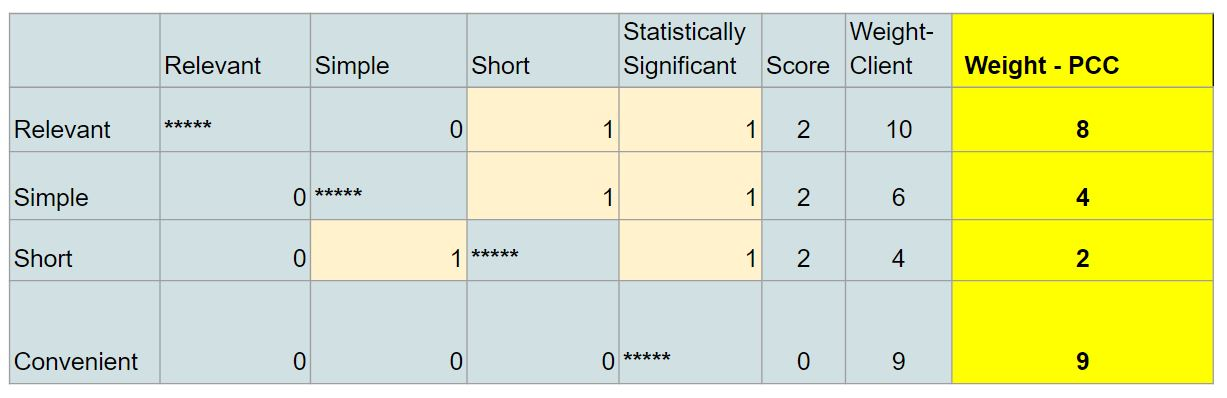
\includegraphics[scale=0.65]{PCC.JPG}
\caption{Pairwise Comparison Chart}
\label{fig:lab}
\end{figure}


\subsection{Metrics}
\par The four highest weighted objectives for our project were simple, short, relevant, and convenient. We weighted each of them from 0-4 based on how they satisfied our customers desired outcomes. For simple, we looked at the level of understanding and training it took to complete the lab and weighted it accordingly. A zero would be extremely difficult, requiring a graduate level education, while a four would require a technical background equivalent to that of a freshman undergraduate student. For short, we gave a time window that it would be acceptable for the lab to last. It would score a zero if it lasted for up to 600 minutes, or 6 lab periods, and a four if it lasted for less than 400 minutes or four lab periods. For the relevancy of the lab, we looked at how the students would be able to learn from this lab as well as achieve decisive results from it. The project would receive a zero if it did not allow the students to test or create a hypothesis as well as not allowing them to achieve decisive results in their reports. A four would be given if they can successfully create and test a hypothesis as well as have decisive results that allow them to reflect on the project in their reports. Lastly, we looked at the convenience of the lab. We ranked it with a zero if the lab caused the professor to spend weeks in advance prepping for the lab, and a four if the lab setup can by achieved by the professor in thirty minutes or less. We believe that with all of these metrics taken into account, we can properly address our problem statement by creating a simple and repeatable lab that teaches students the process of scientific inquiry by studying an organism.






\bibliographystyle{IEEEtran}
\bibliography{roboroach.bib}
\end{document}
